\section{Примеры работы}

Примеры выполнялись на графе,
изображённом на рис. \ref{fig:sample_graph}.

\begin{figure}[H]
    \centering
    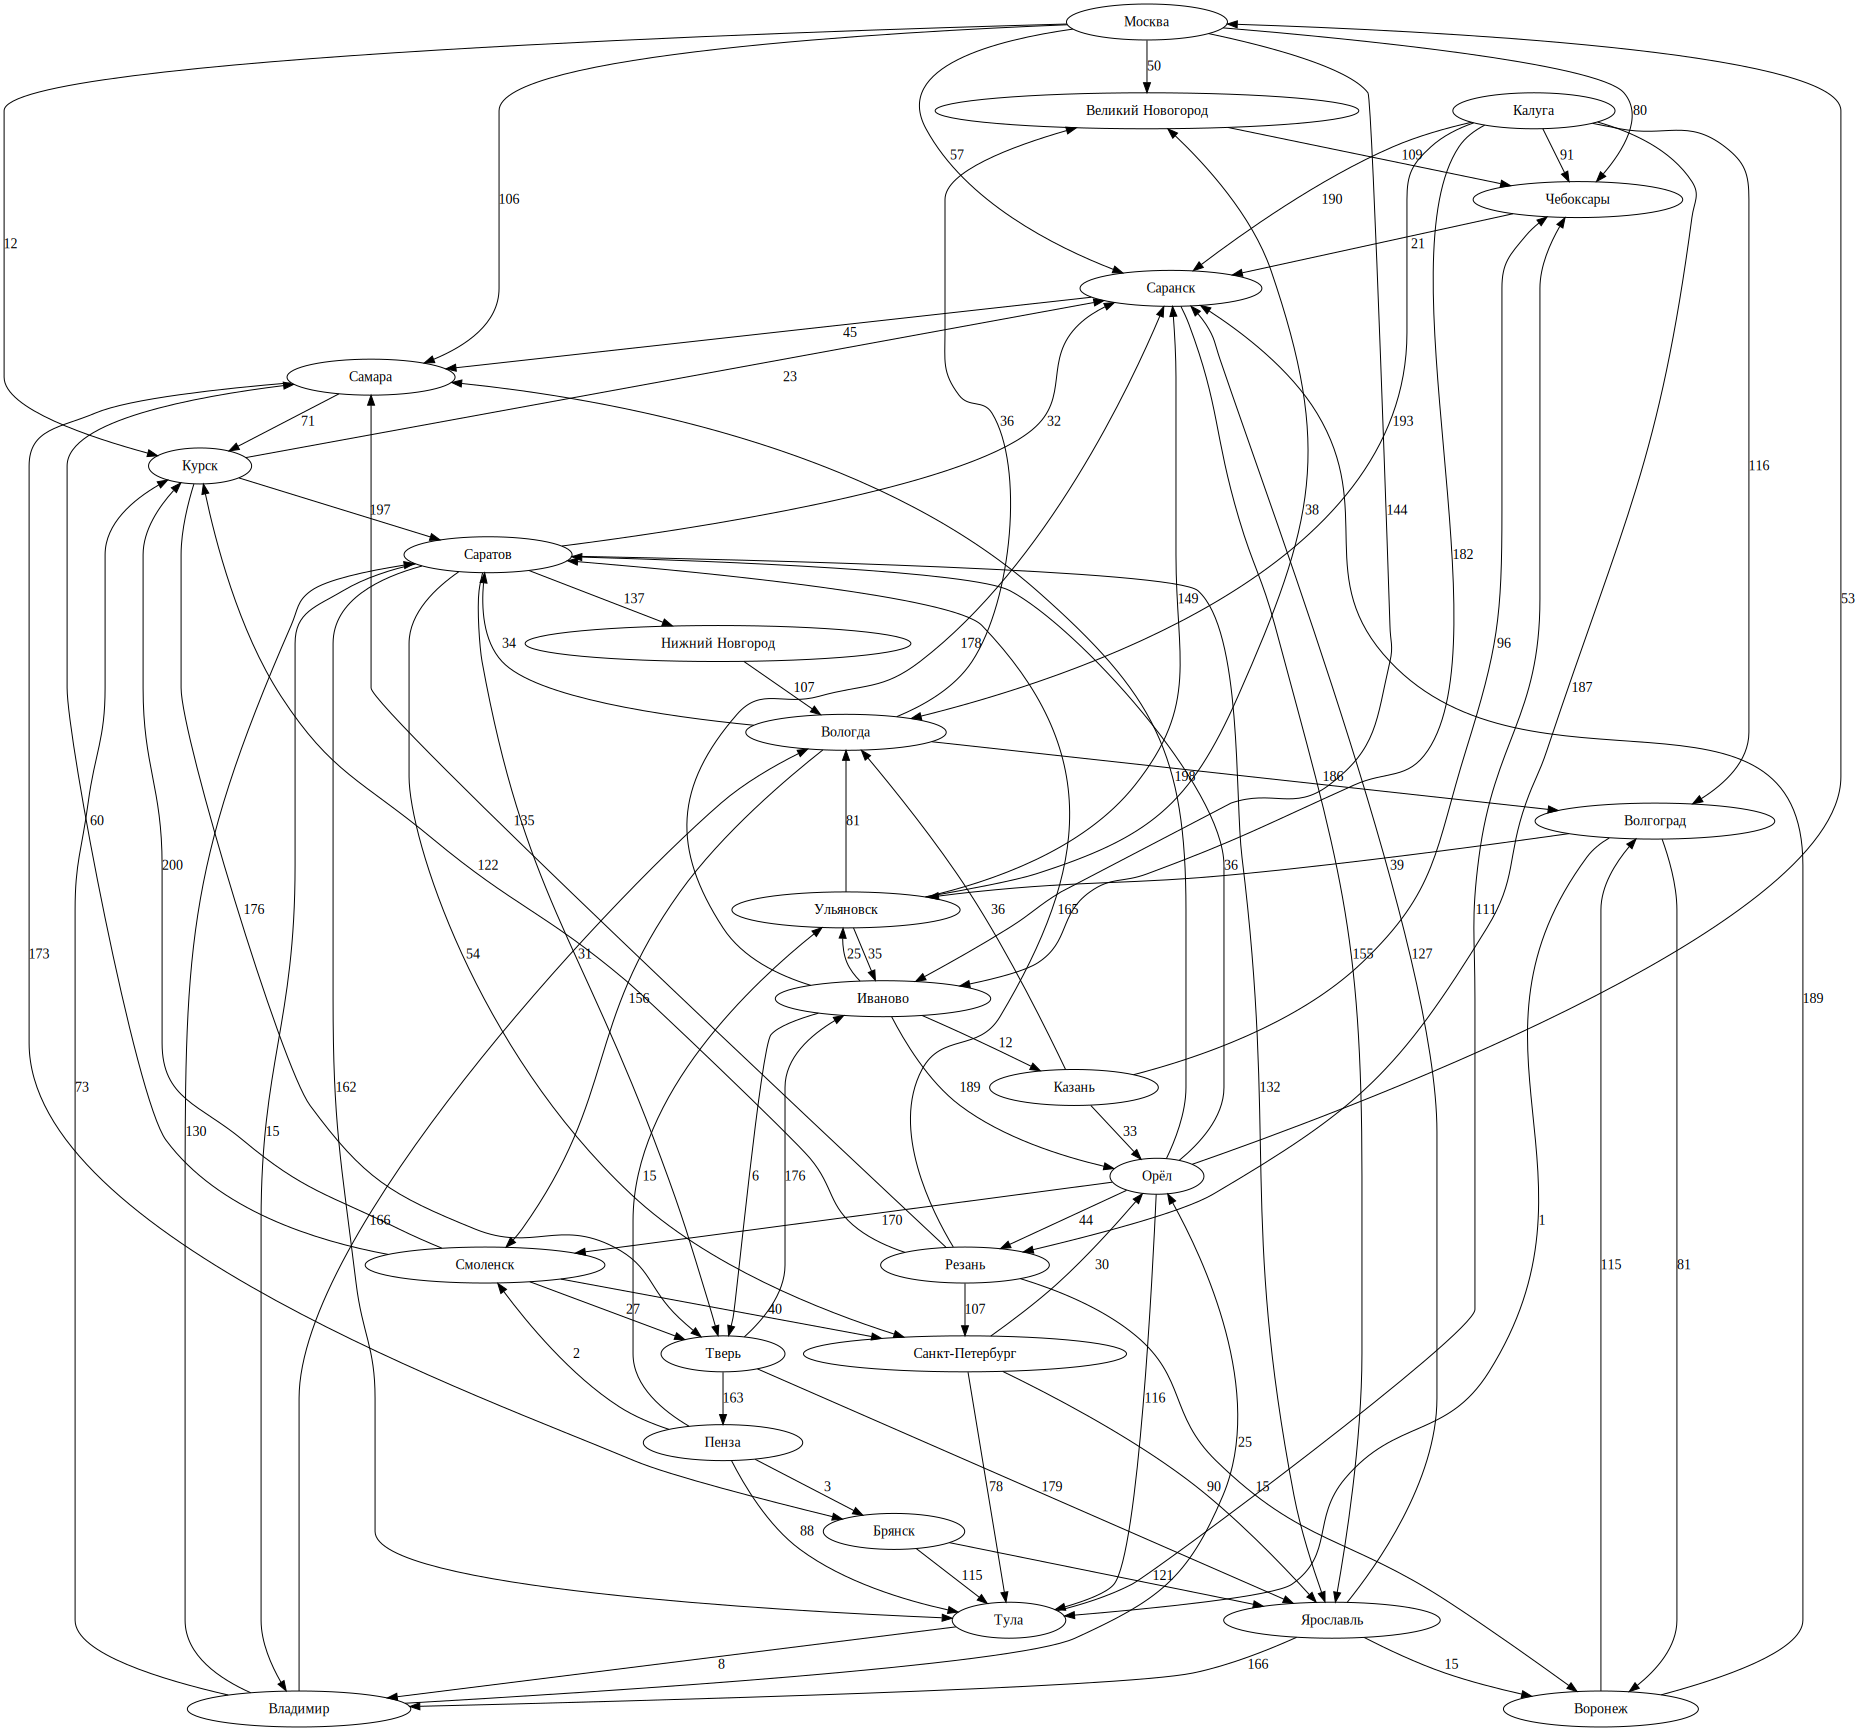
\includegraphics[width=\linewidth]{photo/sample_graph}
    \caption{Граф, использующийся в примерах}
    \label{fig:sample_graph}
\end{figure}

\subsection*{Пример 1}

Стартовый город: Москва

Конечный город: Владимир

Пример выполнения представлен на рис. \ref{fig:example_1}

\begin{figure}[H]
    \centering
    \includegraphics[width=0.7\linewidth]{photo/example_1}
    \caption{Пример выполнения при поиске пути Москва -> Владимир}
    \label{fig:example_1}
\end{figure}

\subsection*{Пример 2}

Стартовый город: Саранск

Конечный город: Воронеж

Пример выполнения представлен на рис. \ref{fig:example_2}

\begin{figure}[H]
    \centering
    \includegraphics[width=0.7\linewidth]{photo/example_2}
    \caption{Пример выполнения при поиске пути Саранск -> Воронеж}
    \label{fig:example_2}
\end{figure}

\subsection*{Пример 3}

Стартовый город: Чебоксары

Конечный город: Иваново

Пример выполнения представлен на рис. \ref{fig:example_3}

\begin{figure}[H]
    \centering
    \includegraphics[width=0.7\linewidth]{photo/example_3}
    \caption{Пример выполнения при поиске пути Чебоксары -> Иваново}
    \label{fig:example_3}
\end{figure}

\subsection*{Пример 4}

Стартовый город: Иваново

Конечный город: Чебоксары

Пример выполнения представлен на рис. \ref{fig:example_4}

\begin{figure}[H]
    \centering
    \includegraphics[width=0.7\linewidth]{photo/example_4}
    \caption{Пример выполнения при поиске пути Иваново -> Чебоксары}
    \label{fig:example_4}
\end{figure}